\documentclass[19pt]{beamer}
\usepackage{graphicx}

% \title{Stereo Vision}
% \author{Robert Washbourne}
% \date{\today}

\begin{document}

% \maketitle

\begin{frame}
\frametitle{Introduction}

Imagine driving in the dark, alert but not noticing a deer crossing the road right in front of you. Using stereo vision methods to see what is close, your car could detect the deer and brake before you even notice the obstacle. \\[15pt]
%
Stereo cameras could find distances, and sensing something closer than 20 feet, send the location to a computer controlling the car. The computer could reason that driving into the obstacle would be catastrophic and turn on the brakes. \\[15pt]
%
The deer, and you, would be safe.
\end{frame}


\begin{frame}
\frametitle{What is stereo matching?}

Stereo matching is a computer technique where two images taken from aligned cameras several centimetres apart are processed for depth information. \\[15pt]
%
For example, taking two images and using a simple algorithm, a colored image is returned, with blue color pixels closer than red color pixels. Here is an example, generated with my code.\\[20pt]

\centering
\setlength\tabcolsep{0.005\textwidth}
\begin{tabular}{ccc}
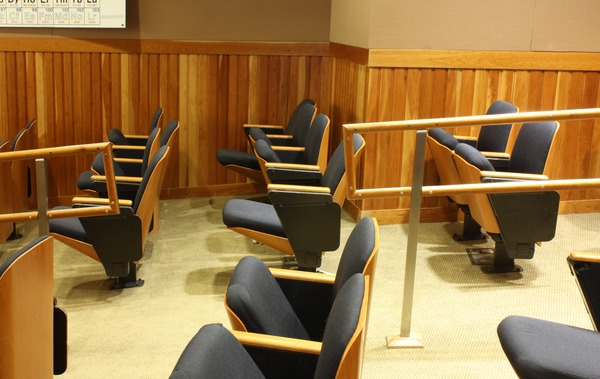
\includegraphics[width=0.33\textwidth]{images/im0-600.jpg} &
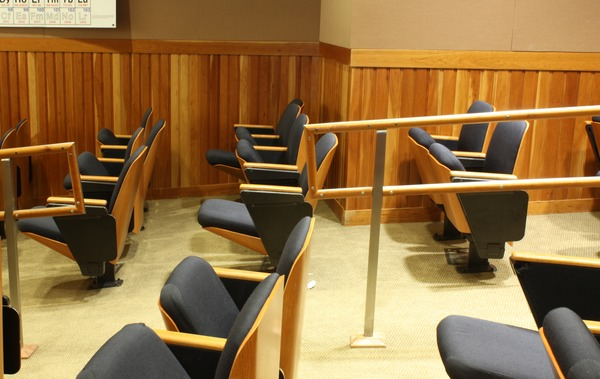
\includegraphics[width=0.33\textwidth]{images/im1-600.jpg} &
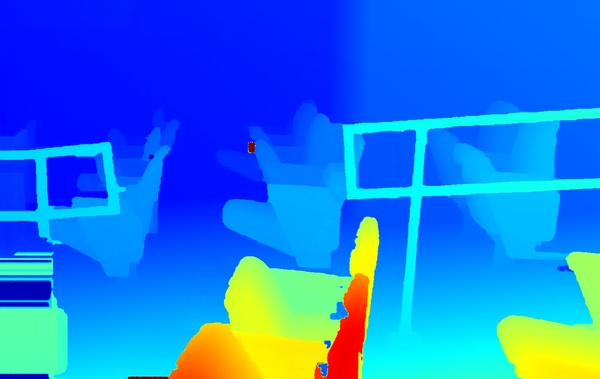
\includegraphics[width=0.33\textwidth]{images/disp-600.jpg} \\[2pt]
Left image & Right Image & Stereo matching \\
\end{tabular}

\end{frame}


\begin{frame}
\frametitle{Program Details}
\begin{enumerate}
    \item Calibrate stereo webcams\\[15pt]
    \item Capture images from stereo webcams\\[15pt]
    \item Split images into one pixel high rows and correlate\\[15pt]
    \item Estimate pixel distance\\[15pt]
    \item Apply edge preserving median filter\\[15pt]
    \item Return the final disparity map 
\end{enumerate}
\end{frame}

\begin{frame}
\frametitle{Workflow 1: Calibrate stereo webcams}

When taking pictures for stereo vision, you need to make sure that the cameras are aligned exactly vertically and horizontally. If they aren't, the disparity map is noisy.\\[15pt]
%
To calibrate two cameras, you print a picture of a chessboard, and using an algorithm called SIFT key point detection, find the corners of the chessboard in both photos.\\[15pt]
%
Once you have the corners as key points, you can find the transformation matrix that maps from the left image to the right image. This will allow perfectly centering the cameras, resulting in  disparity maps with less noise.
\end{frame}

\begin{frame}
\frametitle{Workflow 2: Capture images from stereo webcams}
\end{frame}

\begin{frame}
\frametitle{Workflow 3: Split images into 1 pixel high rows and correlate}
\end{frame}

\begin{frame}
\frametitle{Workflow 1: Estimate pixel distance}
\end{frame}

\begin{frame}
\frametitle{Workflow 1: Apply edge preserving median filter}
\end{frame}

\begin{frame}
\frametitle{Workflow 1: Return the final disparity map}
\end{frame}


\end{document}